% template pour la conversion ipynb → pdf
% author : Pascal Padilla
% source : ???
%
% Deux types de modifications : cellule et page
%   * formatage des cellules : par exemple :
%     '..."metadata": {"tags": ["retenir"]},...'
%       * "cacher"
%       * "exo"
%       * "solution"
%       * "proposition"
%       * "remarque"
%       * "exemple"
%       * "retenir"
%
%   * formatage de la page : theme + titre     
%     ...
%     "metadata": {
%       ...,
%       "latex_metadata": {
%       "theme": "machine",
%       "title": "Représentation des données"
%       },
%     Thèmes possibles : 
%       * "interface"
%       * "machine"
%       * "langage"
%       * "algo"
%       * "struct"
%       * "data"
%       * "reseausocial"
%       * "ds"
%       * "iot"
% 
%
\documentclass[a4paper,17pt]{extarticle}


    %unicode lualatex
\usepackage{fontspec}
\usepackage[sfdefault, condensed]{roboto} % police d'écriture plus moderne
\usepackage[french]{babel} % francisation
\usepackage[parfill]{parskip} %suppression indentation




\usepackage{fancyhdr}
\usepackage{multicol}

% figure non flotantes
\usepackage{float}
\let\origfigure\figure
\let\endorigfigure\endfigure
\renewenvironment{figure}[1][2] {
    \expandafter\origfigure\expandafter[H]
} {
    \endorigfigure
}

% mois/année
\usepackage{datetime}
\newdateformat{monthyeardate}{%
  \monthname[\THEMONTH] \THEYEAR}

% couleurs perso
\usepackage[table]{xcolor}
\definecolor{deepblue}{rgb}{0.3,0.3,0.8}
\definecolor{darkblue}{rgb}{0,0,0.3}
\definecolor{deepred}{rgb}{0.6,0,0}
\definecolor{iremred}{RGB}{204,35,50}
\definecolor{deepgreen}{rgb}{0,0.6,0}
\definecolor{backcolor}{rgb}{0.98,0.95,0.95}
\definecolor{grisClair}{rgb}{0.95,0.95,0.95}
\definecolor{orangeamu}{RGB}{250,178,11}
\definecolor{noiramu}{RGB}{35,31,32}
\definecolor{bleuamu}{RGB}{20,118,198}
\definecolor{bleuamudark}{RGB}{15,90,150}
\definecolor{cyanamu}{RGB}{77,198,244}


\usepackage{/home/bouscadilla/Documents/Code/nbconvert/template/latex/pdf_solution/xeboiboites}
%
% exemple
\newbreakabletheorem[
    small box style={fill=deepblue!90,draw=deepblue!15, rounded corners,line width=1pt},%
    big box style={fill=deepblue!5,draw=deepblue!15,thick,rounded corners,line width=1pt},%
    headfont={\color{white}\bfseries}
        ]{exemple}{Exemple}{}%{counterCo}
%
% remarque
\newbreakabletheorem[
    small box style={draw=ansi-green-intense!100,line width=2pt,fill=ansi-green-intense!0,rounded corners,decoration=penciline, decorate},%
	big box style={color=ansi-green-intense!90,fill=ansi-green-intense!10,thick,decoration={penciline},decorate},
    broken edges={draw=ansi-green-intense!90,thick,fill=orange!20!black!5, decoration={random steps, segment length=.5cm,amplitude=1.3mm},decorate},%
    other edges={decoration=penciline,decorate,thick},%
    headfont={\color{ansi-green-intense}\large\scshape\bfseries}
    ]{remarque}{Remarque}{}%{counterCa}
%
% formule (sans titre)
\newboxedequation[%
    big box style={fill=cyanamu!10,draw=cyanamu!100,thick,decoration=penciline,decorate}]%
    {form}
%
% Réponse
\newbreakabletheorem[
    small box style={fill=bleuamu!100, draw=bleuamu!60, line width=1pt,rounded corners,decorate},%
    big box style={fill=bleuamu!10,draw=bleuamu!30,thick,rounded corners,decorate},
    headfont={\color{white}\large\scshape\bfseries}
        ]{reponse}{Correction}{}
%

%
% À retenir
%\newbreakabletheorem[
%    small box style={fill=deepred!100, draw=deepred!80, line width=1pt,rounded corners,decorate},%
%    big box style={fill=deepred!10,draw=deepred!50,thick,rounded corners,decorate},
%    headfont={\color{white}\large\scshape\bfseries}
%        ]{retenir}{À retenir}{}
%
\newboxedequation[%
    big box style={fill=deepred!10,draw=deepred!0,thick,decoration=penciline,decorate}]%
    {retenir}



% astuce
\newspanning[
    image=/home/bouscadilla/Documents/Code/nbconvert/template/latex/pdf_solution/fig-idee,headfont=\bfseries,
    spanning style={very thick,decoration=penciline,decorate}
    ]{astuce}{Astuce}{}
%
% activité

\newcounter{counterCa}
\newbreakabletheorem[
    small box style={draw=orangeamu!100,line width=2pt,fill=orangeamu!100,rounded corners,decoration=penciline, decorate},%
	big box style={color=orangeamu!100,fill=orangeamu!5,thick,decoration={penciline},decorate},
    broken edges={draw=orangeamu!100,thick,fill=orangeamu!100, decoration={random steps, segment length=.5cm,amplitude=1.3mm},decorate},%
    other edges={decoration=penciline,decorate,thick},%
    headfont={\color{white}\large\scshape\bfseries}
    ]{activite}{\adjustimage{height=1cm, valign=m}{/home/bouscadilla/Documents/Code/nbconvert/template/latex/pdf_solution/papier_eleve_investigation.png}%
    Activité}{counterCa}
%   
%   environnement élève
%
\newenvironment{eleve}%
%{\begin{activite}\large\\} % écrire plus gros
{\begin{activite}\color{noiramu}\\[-0.5cm]}
{\end{activite}}

\newenvironment{formule}%
%{\begin{activite}\large\\} % écrire plus gros
{\begin{form}\color{bleuamu}}
{\end{form}}


\usepackage[breakable]{tcolorbox}
    \usepackage{parskip} % Stop auto-indenting (to mimic markdown behaviour)
    
    \usepackage{iftex}
    \ifPDFTeX
    	\usepackage[T1]{fontenc}
    	\usepackage{mathpazo}
    \else
    	\usepackage{fontspec}
    \fi

    % Basic figure setup, for now with no caption control since it's done
    % automatically by Pandoc (which extracts ![](path) syntax from Markdown).
    \usepackage{graphicx}
    % Maintain compatibility with old templates. Remove in nbconvert 6.0
    \let\Oldincludegraphics\includegraphics
    % Ensure that by default, figures have no caption (until we provide a
    % proper Figure object with a Caption API and a way to capture that
    % in the conversion process - todo).
    \usepackage{caption}
    \DeclareCaptionFormat{nocaption}{}
    \captionsetup{format=nocaption,aboveskip=0pt,belowskip=0pt}

    \usepackage[Export]{adjustbox} % Used to constrain images to a maximum size
    \adjustboxset{max size={0.9\linewidth}{0.9\paperheight}}
    \usepackage{float}
    \floatplacement{figure}{H} % forces figures to be placed at the correct location
    \usepackage{xcolor} % Allow colors to be defined
    \usepackage{enumerate} % Needed for markdown enumerations to work
    \usepackage{geometry} % Used to adjust the document margins
    \usepackage{amsmath} % Equations
    \usepackage{amssymb} % Equations
    \usepackage{textcomp} % defines textquotesingle
    % Hack from http://tex.stackexchange.com/a/47451/13684:
    \AtBeginDocument{%
        \def\PYZsq{\textquotesingle}% Upright quotes in Pygmentized code
    }
    \usepackage{upquote} % Upright quotes for verbatim code
    \usepackage{eurosym} % defines \euro
    \usepackage[mathletters]{ucs} % Extended unicode (utf-8) support
    \usepackage{fancyvrb} % verbatim replacement that allows latex

    % The hyperref package gives us a pdf with properly built
    % internal navigation ('pdf bookmarks' for the table of contents,
    % internal cross-reference links, web links for URLs, etc.)
    \usepackage{hyperref}
    % The default LaTeX title has an obnoxious amount of whitespace. By default,
    % titling removes some of it. It also provides customization options.
    \usepackage{titling}
    \usepackage{longtable} % longtable support required by pandoc >1.10
    \usepackage{booktabs}  % table support for pandoc > 1.12.2
    \usepackage[inline]{enumitem} % IRkernel/repr support (it uses the enumerate* environment)
    \usepackage[normalem]{ulem} % ulem is needed to support strikethroughs (\sout)
                                % normalem makes italics be italics, not underlines
    \usepackage{mathrsfs}
    

    
    % Colors for the hyperref package
    \definecolor{urlcolor}{rgb}{0,.145,.698}
    \definecolor{linkcolor}{rgb}{.71,0.21,0.01}
    \definecolor{citecolor}{rgb}{.12,.54,.11}

    % ANSI colors
    \definecolor{ansi-black}{HTML}{3E424D}
    \definecolor{ansi-black-intense}{HTML}{282C36}
    \definecolor{ansi-red}{HTML}{E75C58}
    \definecolor{ansi-red-intense}{HTML}{B22B31}
    \definecolor{ansi-green}{HTML}{00A250}
    \definecolor{ansi-green-intense}{HTML}{007427}
    \definecolor{ansi-yellow}{HTML}{DDB62B}
    \definecolor{ansi-yellow-intense}{HTML}{B27D12}
    \definecolor{ansi-blue}{HTML}{208FFB}
    \definecolor{ansi-blue-intense}{HTML}{0065CA}
    \definecolor{ansi-magenta}{HTML}{D160C4}
    \definecolor{ansi-magenta-intense}{HTML}{A03196}
    \definecolor{ansi-cyan}{HTML}{60C6C8}
    \definecolor{ansi-cyan-intense}{HTML}{258F8F}
    \definecolor{ansi-white}{HTML}{C5C1B4}
    \definecolor{ansi-white-intense}{HTML}{A1A6B2}
    \definecolor{ansi-default-inverse-fg}{HTML}{FFFFFF}
    \definecolor{ansi-default-inverse-bg}{HTML}{000000}

    % commands and environments needed by pandoc snippets
    % extracted from the output of `pandoc -s`
    \providecommand{\tightlist}{%
      \setlength{\itemsep}{0pt}\setlength{\parskip}{0pt}}
    \DefineVerbatimEnvironment{Highlighting}{Verbatim}{commandchars=\\\{\}}
    % Add ',fontsize=\small' for more characters per line
    \newenvironment{Shaded}{}{}
    \newcommand{\KeywordTok}[1]{\textcolor[rgb]{0.00,0.44,0.13}{\textbf{{#1}}}}
    \newcommand{\DataTypeTok}[1]{\textcolor[rgb]{0.56,0.13,0.00}{{#1}}}
    \newcommand{\DecValTok}[1]{\textcolor[rgb]{0.25,0.63,0.44}{{#1}}}
    \newcommand{\BaseNTok}[1]{\textcolor[rgb]{0.25,0.63,0.44}{{#1}}}
    \newcommand{\FloatTok}[1]{\textcolor[rgb]{0.25,0.63,0.44}{{#1}}}
    \newcommand{\CharTok}[1]{\textcolor[rgb]{0.25,0.44,0.63}{{#1}}}
    \newcommand{\StringTok}[1]{\textcolor[rgb]{0.25,0.44,0.63}{{#1}}}
    \newcommand{\CommentTok}[1]{\textcolor[rgb]{0.38,0.63,0.69}{\textit{{#1}}}}
    \newcommand{\OtherTok}[1]{\textcolor[rgb]{0.00,0.44,0.13}{{#1}}}
    \newcommand{\AlertTok}[1]{\textcolor[rgb]{1.00,0.00,0.00}{\textbf{{#1}}}}
    \newcommand{\FunctionTok}[1]{\textcolor[rgb]{0.02,0.16,0.49}{{#1}}}
    \newcommand{\RegionMarkerTok}[1]{{#1}}
    \newcommand{\ErrorTok}[1]{\textcolor[rgb]{1.00,0.00,0.00}{\textbf{{#1}}}}
    \newcommand{\NormalTok}[1]{{#1}}
    
    % Additional commands for more recent versions of Pandoc
    \newcommand{\ConstantTok}[1]{\textcolor[rgb]{0.53,0.00,0.00}{{#1}}}
    \newcommand{\SpecialCharTok}[1]{\textcolor[rgb]{0.25,0.44,0.63}{{#1}}}
    \newcommand{\VerbatimStringTok}[1]{\textcolor[rgb]{0.25,0.44,0.63}{{#1}}}
    \newcommand{\SpecialStringTok}[1]{\textcolor[rgb]{0.73,0.40,0.53}{{#1}}}
    \newcommand{\ImportTok}[1]{{#1}}
    \newcommand{\DocumentationTok}[1]{\textcolor[rgb]{0.73,0.13,0.13}{\textit{{#1}}}}
    \newcommand{\AnnotationTok}[1]{\textcolor[rgb]{0.38,0.63,0.69}{\textbf{\textit{{#1}}}}}
    \newcommand{\CommentVarTok}[1]{\textcolor[rgb]{0.38,0.63,0.69}{\textbf{\textit{{#1}}}}}
    \newcommand{\VariableTok}[1]{\textcolor[rgb]{0.10,0.09,0.49}{{#1}}}
    \newcommand{\ControlFlowTok}[1]{\textcolor[rgb]{0.00,0.44,0.13}{\textbf{{#1}}}}
    \newcommand{\OperatorTok}[1]{\textcolor[rgb]{0.40,0.40,0.40}{{#1}}}
    \newcommand{\BuiltInTok}[1]{{#1}}
    \newcommand{\ExtensionTok}[1]{{#1}}
    \newcommand{\PreprocessorTok}[1]{\textcolor[rgb]{0.74,0.48,0.00}{{#1}}}
    \newcommand{\AttributeTok}[1]{\textcolor[rgb]{0.49,0.56,0.16}{{#1}}}
    \newcommand{\InformationTok}[1]{\textcolor[rgb]{0.38,0.63,0.69}{\textbf{\textit{{#1}}}}}
    \newcommand{\WarningTok}[1]{\textcolor[rgb]{0.38,0.63,0.69}{\textbf{\textit{{#1}}}}}
    
    
    % Define a nice break command that doesn't care if a line doesn't already
    % exist.
    \def\br{\hspace*{\fill} \\* }
    % Math Jax compatibility definitions
    \def\gt{>}
    \def\lt{<}
    \let\Oldtex\TeX
    \let\Oldlatex\LaTeX
    \renewcommand{\TeX}{\textrm{\Oldtex}}
    \renewcommand{\LaTeX}{\textrm{\Oldlatex}}
    % Document parameters
    % Document title
    \title{2-7-1---basesPython-Fonction}
    
    
    
    
    
% Pygments definitions
\makeatletter
\def\PY@reset{\let\PY@it=\relax \let\PY@bf=\relax%
    \let\PY@ul=\relax \let\PY@tc=\relax%
    \let\PY@bc=\relax \let\PY@ff=\relax}
\def\PY@tok#1{\csname PY@tok@#1\endcsname}
\def\PY@toks#1+{\ifx\relax#1\empty\else%
    \PY@tok{#1}\expandafter\PY@toks\fi}
\def\PY@do#1{\PY@bc{\PY@tc{\PY@ul{%
    \PY@it{\PY@bf{\PY@ff{#1}}}}}}}
\def\PY#1#2{\PY@reset\PY@toks#1+\relax+\PY@do{#2}}

\expandafter\def\csname PY@tok@w\endcsname{\def\PY@tc##1{\textcolor[rgb]{0.73,0.73,0.73}{##1}}}
\expandafter\def\csname PY@tok@c\endcsname{\let\PY@it=\textit\def\PY@tc##1{\textcolor[rgb]{0.25,0.50,0.50}{##1}}}
\expandafter\def\csname PY@tok@cp\endcsname{\def\PY@tc##1{\textcolor[rgb]{0.74,0.48,0.00}{##1}}}
\expandafter\def\csname PY@tok@k\endcsname{\let\PY@bf=\textbf\def\PY@tc##1{\textcolor[rgb]{0.00,0.50,0.00}{##1}}}
\expandafter\def\csname PY@tok@kp\endcsname{\def\PY@tc##1{\textcolor[rgb]{0.00,0.50,0.00}{##1}}}
\expandafter\def\csname PY@tok@kt\endcsname{\def\PY@tc##1{\textcolor[rgb]{0.69,0.00,0.25}{##1}}}
\expandafter\def\csname PY@tok@o\endcsname{\def\PY@tc##1{\textcolor[rgb]{0.40,0.40,0.40}{##1}}}
\expandafter\def\csname PY@tok@ow\endcsname{\let\PY@bf=\textbf\def\PY@tc##1{\textcolor[rgb]{0.67,0.13,1.00}{##1}}}
\expandafter\def\csname PY@tok@nb\endcsname{\def\PY@tc##1{\textcolor[rgb]{0.00,0.50,0.00}{##1}}}
\expandafter\def\csname PY@tok@nf\endcsname{\def\PY@tc##1{\textcolor[rgb]{0.00,0.00,1.00}{##1}}}
\expandafter\def\csname PY@tok@nc\endcsname{\let\PY@bf=\textbf\def\PY@tc##1{\textcolor[rgb]{0.00,0.00,1.00}{##1}}}
\expandafter\def\csname PY@tok@nn\endcsname{\let\PY@bf=\textbf\def\PY@tc##1{\textcolor[rgb]{0.00,0.00,1.00}{##1}}}
\expandafter\def\csname PY@tok@ne\endcsname{\let\PY@bf=\textbf\def\PY@tc##1{\textcolor[rgb]{0.82,0.25,0.23}{##1}}}
\expandafter\def\csname PY@tok@nv\endcsname{\def\PY@tc##1{\textcolor[rgb]{0.10,0.09,0.49}{##1}}}
\expandafter\def\csname PY@tok@no\endcsname{\def\PY@tc##1{\textcolor[rgb]{0.53,0.00,0.00}{##1}}}
\expandafter\def\csname PY@tok@nl\endcsname{\def\PY@tc##1{\textcolor[rgb]{0.63,0.63,0.00}{##1}}}
\expandafter\def\csname PY@tok@ni\endcsname{\let\PY@bf=\textbf\def\PY@tc##1{\textcolor[rgb]{0.60,0.60,0.60}{##1}}}
\expandafter\def\csname PY@tok@na\endcsname{\def\PY@tc##1{\textcolor[rgb]{0.49,0.56,0.16}{##1}}}
\expandafter\def\csname PY@tok@nt\endcsname{\let\PY@bf=\textbf\def\PY@tc##1{\textcolor[rgb]{0.00,0.50,0.00}{##1}}}
\expandafter\def\csname PY@tok@nd\endcsname{\def\PY@tc##1{\textcolor[rgb]{0.67,0.13,1.00}{##1}}}
\expandafter\def\csname PY@tok@s\endcsname{\def\PY@tc##1{\textcolor[rgb]{0.73,0.13,0.13}{##1}}}
\expandafter\def\csname PY@tok@sd\endcsname{\let\PY@it=\textit\def\PY@tc##1{\textcolor[rgb]{0.73,0.13,0.13}{##1}}}
\expandafter\def\csname PY@tok@si\endcsname{\let\PY@bf=\textbf\def\PY@tc##1{\textcolor[rgb]{0.73,0.40,0.53}{##1}}}
\expandafter\def\csname PY@tok@se\endcsname{\let\PY@bf=\textbf\def\PY@tc##1{\textcolor[rgb]{0.73,0.40,0.13}{##1}}}
\expandafter\def\csname PY@tok@sr\endcsname{\def\PY@tc##1{\textcolor[rgb]{0.73,0.40,0.53}{##1}}}
\expandafter\def\csname PY@tok@ss\endcsname{\def\PY@tc##1{\textcolor[rgb]{0.10,0.09,0.49}{##1}}}
\expandafter\def\csname PY@tok@sx\endcsname{\def\PY@tc##1{\textcolor[rgb]{0.00,0.50,0.00}{##1}}}
\expandafter\def\csname PY@tok@m\endcsname{\def\PY@tc##1{\textcolor[rgb]{0.40,0.40,0.40}{##1}}}
\expandafter\def\csname PY@tok@gh\endcsname{\let\PY@bf=\textbf\def\PY@tc##1{\textcolor[rgb]{0.00,0.00,0.50}{##1}}}
\expandafter\def\csname PY@tok@gu\endcsname{\let\PY@bf=\textbf\def\PY@tc##1{\textcolor[rgb]{0.50,0.00,0.50}{##1}}}
\expandafter\def\csname PY@tok@gd\endcsname{\def\PY@tc##1{\textcolor[rgb]{0.63,0.00,0.00}{##1}}}
\expandafter\def\csname PY@tok@gi\endcsname{\def\PY@tc##1{\textcolor[rgb]{0.00,0.63,0.00}{##1}}}
\expandafter\def\csname PY@tok@gr\endcsname{\def\PY@tc##1{\textcolor[rgb]{1.00,0.00,0.00}{##1}}}
\expandafter\def\csname PY@tok@ge\endcsname{\let\PY@it=\textit}
\expandafter\def\csname PY@tok@gs\endcsname{\let\PY@bf=\textbf}
\expandafter\def\csname PY@tok@gp\endcsname{\let\PY@bf=\textbf\def\PY@tc##1{\textcolor[rgb]{0.00,0.00,0.50}{##1}}}
\expandafter\def\csname PY@tok@go\endcsname{\def\PY@tc##1{\textcolor[rgb]{0.53,0.53,0.53}{##1}}}
\expandafter\def\csname PY@tok@gt\endcsname{\def\PY@tc##1{\textcolor[rgb]{0.00,0.27,0.87}{##1}}}
\expandafter\def\csname PY@tok@err\endcsname{\def\PY@bc##1{\setlength{\fboxsep}{0pt}\fcolorbox[rgb]{1.00,0.00,0.00}{1,1,1}{\strut ##1}}}
\expandafter\def\csname PY@tok@kc\endcsname{\let\PY@bf=\textbf\def\PY@tc##1{\textcolor[rgb]{0.00,0.50,0.00}{##1}}}
\expandafter\def\csname PY@tok@kd\endcsname{\let\PY@bf=\textbf\def\PY@tc##1{\textcolor[rgb]{0.00,0.50,0.00}{##1}}}
\expandafter\def\csname PY@tok@kn\endcsname{\let\PY@bf=\textbf\def\PY@tc##1{\textcolor[rgb]{0.00,0.50,0.00}{##1}}}
\expandafter\def\csname PY@tok@kr\endcsname{\let\PY@bf=\textbf\def\PY@tc##1{\textcolor[rgb]{0.00,0.50,0.00}{##1}}}
\expandafter\def\csname PY@tok@bp\endcsname{\def\PY@tc##1{\textcolor[rgb]{0.00,0.50,0.00}{##1}}}
\expandafter\def\csname PY@tok@fm\endcsname{\def\PY@tc##1{\textcolor[rgb]{0.00,0.00,1.00}{##1}}}
\expandafter\def\csname PY@tok@vc\endcsname{\def\PY@tc##1{\textcolor[rgb]{0.10,0.09,0.49}{##1}}}
\expandafter\def\csname PY@tok@vg\endcsname{\def\PY@tc##1{\textcolor[rgb]{0.10,0.09,0.49}{##1}}}
\expandafter\def\csname PY@tok@vi\endcsname{\def\PY@tc##1{\textcolor[rgb]{0.10,0.09,0.49}{##1}}}
\expandafter\def\csname PY@tok@vm\endcsname{\def\PY@tc##1{\textcolor[rgb]{0.10,0.09,0.49}{##1}}}
\expandafter\def\csname PY@tok@sa\endcsname{\def\PY@tc##1{\textcolor[rgb]{0.73,0.13,0.13}{##1}}}
\expandafter\def\csname PY@tok@sb\endcsname{\def\PY@tc##1{\textcolor[rgb]{0.73,0.13,0.13}{##1}}}
\expandafter\def\csname PY@tok@sc\endcsname{\def\PY@tc##1{\textcolor[rgb]{0.73,0.13,0.13}{##1}}}
\expandafter\def\csname PY@tok@dl\endcsname{\def\PY@tc##1{\textcolor[rgb]{0.73,0.13,0.13}{##1}}}
\expandafter\def\csname PY@tok@s2\endcsname{\def\PY@tc##1{\textcolor[rgb]{0.73,0.13,0.13}{##1}}}
\expandafter\def\csname PY@tok@sh\endcsname{\def\PY@tc##1{\textcolor[rgb]{0.73,0.13,0.13}{##1}}}
\expandafter\def\csname PY@tok@s1\endcsname{\def\PY@tc##1{\textcolor[rgb]{0.73,0.13,0.13}{##1}}}
\expandafter\def\csname PY@tok@mb\endcsname{\def\PY@tc##1{\textcolor[rgb]{0.40,0.40,0.40}{##1}}}
\expandafter\def\csname PY@tok@mf\endcsname{\def\PY@tc##1{\textcolor[rgb]{0.40,0.40,0.40}{##1}}}
\expandafter\def\csname PY@tok@mh\endcsname{\def\PY@tc##1{\textcolor[rgb]{0.40,0.40,0.40}{##1}}}
\expandafter\def\csname PY@tok@mi\endcsname{\def\PY@tc##1{\textcolor[rgb]{0.40,0.40,0.40}{##1}}}
\expandafter\def\csname PY@tok@il\endcsname{\def\PY@tc##1{\textcolor[rgb]{0.40,0.40,0.40}{##1}}}
\expandafter\def\csname PY@tok@mo\endcsname{\def\PY@tc##1{\textcolor[rgb]{0.40,0.40,0.40}{##1}}}
\expandafter\def\csname PY@tok@ch\endcsname{\let\PY@it=\textit\def\PY@tc##1{\textcolor[rgb]{0.25,0.50,0.50}{##1}}}
\expandafter\def\csname PY@tok@cm\endcsname{\let\PY@it=\textit\def\PY@tc##1{\textcolor[rgb]{0.25,0.50,0.50}{##1}}}
\expandafter\def\csname PY@tok@cpf\endcsname{\let\PY@it=\textit\def\PY@tc##1{\textcolor[rgb]{0.25,0.50,0.50}{##1}}}
\expandafter\def\csname PY@tok@c1\endcsname{\let\PY@it=\textit\def\PY@tc##1{\textcolor[rgb]{0.25,0.50,0.50}{##1}}}
\expandafter\def\csname PY@tok@cs\endcsname{\let\PY@it=\textit\def\PY@tc##1{\textcolor[rgb]{0.25,0.50,0.50}{##1}}}

\def\PYZbs{\char`\\}
\def\PYZus{\char`\_}
\def\PYZob{\char`\{}
\def\PYZcb{\char`\}}
\def\PYZca{\char`\^}
\def\PYZam{\char`\&}
\def\PYZlt{\char`\<}
\def\PYZgt{\char`\>}
\def\PYZsh{\char`\#}
\def\PYZpc{\char`\%}
\def\PYZdl{\char`\$}
\def\PYZhy{\char`\-}
\def\PYZsq{\char`\'}
\def\PYZdq{\char`\"}
\def\PYZti{\char`\~}
% for compatibility with earlier versions
\def\PYZat{@}
\def\PYZlb{[}
\def\PYZrb{]}
\makeatother


    % For linebreaks inside Verbatim environment from package fancyvrb. 
    \makeatletter
        \newbox\Wrappedcontinuationbox 
        \newbox\Wrappedvisiblespacebox 
        \newcommand*\Wrappedvisiblespace {\textcolor{red}{\textvisiblespace}} 
        \newcommand*\Wrappedcontinuationsymbol {\textcolor{red}{\llap{\tiny$\m@th\hookrightarrow$}}} 
        \newcommand*\Wrappedcontinuationindent {3ex } 
        \newcommand*\Wrappedafterbreak {\kern\Wrappedcontinuationindent\copy\Wrappedcontinuationbox} 
        % Take advantage of the already applied Pygments mark-up to insert 
        % potential linebreaks for TeX processing. 
        %        {, <, #, %, $, ' and ": go to next line. 
        %        _, }, ^, &, >, - and ~: stay at end of broken line. 
        % Use of \textquotesingle for straight quote. 
        \newcommand*\Wrappedbreaksatspecials {% 
            \def\PYGZus{\discretionary{\char`\_}{\Wrappedafterbreak}{\char`\_}}% 
            \def\PYGZob{\discretionary{}{\Wrappedafterbreak\char`\{}{\char`\{}}% 
            \def\PYGZcb{\discretionary{\char`\}}{\Wrappedafterbreak}{\char`\}}}% 
            \def\PYGZca{\discretionary{\char`\^}{\Wrappedafterbreak}{\char`\^}}% 
            \def\PYGZam{\discretionary{\char`\&}{\Wrappedafterbreak}{\char`\&}}% 
            \def\PYGZlt{\discretionary{}{\Wrappedafterbreak\char`\<}{\char`\<}}% 
            \def\PYGZgt{\discretionary{\char`\>}{\Wrappedafterbreak}{\char`\>}}% 
            \def\PYGZsh{\discretionary{}{\Wrappedafterbreak\char`\#}{\char`\#}}% 
            \def\PYGZpc{\discretionary{}{\Wrappedafterbreak\char`\%}{\char`\%}}% 
            \def\PYGZdl{\discretionary{}{\Wrappedafterbreak\char`\$}{\char`\$}}% 
            \def\PYGZhy{\discretionary{\char`\-}{\Wrappedafterbreak}{\char`\-}}% 
            \def\PYGZsq{\discretionary{}{\Wrappedafterbreak\textquotesingle}{\textquotesingle}}% 
            \def\PYGZdq{\discretionary{}{\Wrappedafterbreak\char`\"}{\char`\"}}% 
            \def\PYGZti{\discretionary{\char`\~}{\Wrappedafterbreak}{\char`\~}}% 
        } 
        % Some characters . , ; ? ! / are not pygmentized. 
        % This macro makes them "active" and they will insert potential linebreaks 
        \newcommand*\Wrappedbreaksatpunct {% 
            \lccode`\~`\.\lowercase{\def~}{\discretionary{\hbox{\char`\.}}{\Wrappedafterbreak}{\hbox{\char`\.}}}% 
            \lccode`\~`\,\lowercase{\def~}{\discretionary{\hbox{\char`\,}}{\Wrappedafterbreak}{\hbox{\char`\,}}}% 
            \lccode`\~`\;\lowercase{\def~}{\discretionary{\hbox{\char`\;}}{\Wrappedafterbreak}{\hbox{\char`\;}}}% 
            \lccode`\~`\:\lowercase{\def~}{\discretionary{\hbox{\char`\:}}{\Wrappedafterbreak}{\hbox{\char`\:}}}% 
            \lccode`\~`\?\lowercase{\def~}{\discretionary{\hbox{\char`\?}}{\Wrappedafterbreak}{\hbox{\char`\?}}}% 
            \lccode`\~`\!\lowercase{\def~}{\discretionary{\hbox{\char`\!}}{\Wrappedafterbreak}{\hbox{\char`\!}}}% 
            \lccode`\~`\/\lowercase{\def~}{\discretionary{\hbox{\char`\/}}{\Wrappedafterbreak}{\hbox{\char`\/}}}% 
            \catcode`\.\active
            \catcode`\,\active 
            \catcode`\;\active
            \catcode`\:\active
            \catcode`\?\active
            \catcode`\!\active
            \catcode`\/\active 
            \lccode`\~`\~ 	
        }
    \makeatother

    \let\OriginalVerbatim=\Verbatim
    \makeatletter
    \renewcommand{\Verbatim}[1][1]{%
        %\parskip\z@skip
        \sbox\Wrappedcontinuationbox {\Wrappedcontinuationsymbol}%
        \sbox\Wrappedvisiblespacebox {\FV@SetupFont\Wrappedvisiblespace}%
        \def\FancyVerbFormatLine ##1{\hsize\linewidth
            \vtop{\raggedright\hyphenpenalty\z@\exhyphenpenalty\z@
                \doublehyphendemerits\z@\finalhyphendemerits\z@
                \strut ##1\strut}%
        }%
        % If the linebreak is at a space, the latter will be displayed as visible
        % space at end of first line, and a continuation symbol starts next line.
        % Stretch/shrink are however usually zero for typewriter font.
        \def\FV@Space {%
            \nobreak\hskip\z@ plus\fontdimen3\font minus\fontdimen4\font
            \discretionary{\copy\Wrappedvisiblespacebox}{\Wrappedafterbreak}
            {\kern\fontdimen2\font}%
        }%
        
        % Allow breaks at special characters using \PYG... macros.
        \Wrappedbreaksatspecials
        % Breaks at punctuation characters . , ; ? ! and / need catcode=\active 	
        \OriginalVerbatim[#1,codes*=\Wrappedbreaksatpunct]%
    }
    \makeatother

    % Exact colors from NB
    \definecolor{incolor}{HTML}{303F9F}
    \definecolor{outcolor}{HTML}{D84315}
    \definecolor{cellborder}{HTML}{CFCFCF}
    \definecolor{cellbackground}{HTML}{F7F7F7}
    
    % prompt
    \makeatletter
    \newcommand{\boxspacing}{\kern\kvtcb@left@rule\kern\kvtcb@boxsep}
    \makeatother
    \newcommand{\prompt}[4]{
        \ttfamily\llap{{\color{#2}[#3]:\hspace{3pt}#4}}\vspace{-\baselineskip}
    }
    

    
\setlength\headheight{30pt}
\setcounter{secnumdepth}{0} % Turns off numbering for sections

    % Prevent overflowing lines due to hard-to-break entities
    \sloppy 
    % Setup hyperref package
    \hypersetup{
      breaklinks=true,  % so long urls are correctly broken across lines
      colorlinks=true,
      urlcolor=urlcolor,
      linkcolor=linkcolor,
      citecolor=citecolor,
      }
    % Slightly bigger margins than the latex defaults
    \geometry{a4paper,tmargin=3cm,bmargin=2cm,lmargin=1cm,rmargin=1cm}\fancyhead[L]{Thème à définir}\fancyhead[L]{\adjustimage{height=1cm, valign=m}{/home/bouscadilla/Documents/Code/nbconvert/template/latex/pdf_solution/papier_eleve_ico_langage}\ttfamily\scshape Langage}\fancyhead[C]{\bfseries\MakeUppercase{2-7-1---basesPython-Fonction}}\fancyhead[C]{\bfseries\MakeUppercase{2.7 --- Programmer en Python}}\fancyhead[R]{décembre 2021}

    \fancyfoot[C]{\thepage}
    % #TODO ajouter les pages totales

    \pagestyle{fancy}
    


\begin{document}
    
    \title{2.7 --- Programmer en Python}
% \maketitle

    
    

    
    \hypertarget{fonctions}{%
\subsection{7 --- Fonctions}\label{fonctions}}

    \hypertarget{introduction}{%
\subsubsection{Introduction}\label{introduction}}
\begin{eleve}
    On souhaite réaliser une application. Lors de l'exécution de notre
application, avant d'arriver à l'écran de menus, il est habituel
d'afficher un écran d'accueil appelé \emph{splash screen} affichant le
nom de l'application, une référence à l'équipe de production.

L'application affiche un écran d'accueil le nom de l'application, sa
version et le nom de l'équipe de production. Après le chargement des
données, on indiquera à l'utilisateur qu'il doit appuyer sur
\texttt{Entrée} pour passer à la suite. Lorsque l'utilisateur valide,
afficher un menu (par exemple \texttt{"Nouvelle\ Partie"},
\texttt{"Sauvegardes"}, \texttt{"Configuration"}).
        
        \end{eleve}\begin{reponse}
    Le programme réalisé est peu satisfaisant. Il comporte clairement trois
grandes parties différentes mais tout est écrit en un seul bloc. Il
serait pratique de structurer le code en trois sous fonctionnalités :

\begin{itemize}
\tightlist
\item
  \texttt{afficher\_splash},
\item
  \texttt{charger\_data} et
\item
  \texttt{afficher\_menu}.
\end{itemize}

        \end{reponse}
    Nous allons voir dans cette leçon comment rendre le code plus élégant en
définissant des \textbf{fonctions}, c'est à dire des fragments de codes
réutilisables réalisant une tâche donnée pouvant dépendre d'un certain
nombre de paramètres.

    \hypertarget{duxe9finir-une-fonction}{%
\subsubsection{Définir une fonction}\label{duxe9finir-une-fonction}}

    Une fonction associe une séquence d'instructions à un nom.
\begin{exemple}
    \textbf{Suite de l'activité 1.} Voici par exemple un exemple simple
d'une fonction \texttt{afficher\_menu} qui affiche un menu composé de
trois lignes : \texttt{"Nouvelle\ Partie"}, \texttt{"Sauvegardes"},
\texttt{"Configuration"}.

\begin{Shaded}
\begin{Highlighting}[]
\KeywordTok{def}\NormalTok{ afficher\_menu():}
    \BuiltInTok{print}\NormalTok{(}\StringTok{"==============="}\NormalTok{)}
    \BuiltInTok{print}\NormalTok{(}\StringTok{"Nouvelle Partie"}\NormalTok{)}
    \BuiltInTok{print}\NormalTok{(}\StringTok{"{-}{-}{-}{-}{-}{-}{-}{-}{-}{-}{-}{-}{-}{-}{-}"}\NormalTok{)}
    \BuiltInTok{print}\NormalTok{(}\StringTok{"  Sauvegardes"}\NormalTok{)}
    \BuiltInTok{print}\NormalTok{(}\StringTok{"{-}{-}{-}{-}{-}{-}{-}{-}{-}{-}{-}{-}{-}{-}{-}"}\NormalTok{)}
    \BuiltInTok{print}\NormalTok{(}\StringTok{" Configuration"}\NormalTok{)}
    \BuiltInTok{print}\NormalTok{(}\StringTok{"==============="}\NormalTok{)}
\end{Highlighting}
\end{Shaded}

        \end{exemple}\begin{retenir}
    La \textbf{définition} commence par

\begin{itemize}
\tightlist
\item
  le mot-clé \texttt{def}, suivi par
\item
  le nom de la fonction (ici \texttt{afficher\_menu}), puis
\item
  une paire de parenthèses et
\item
  deux points.
\end{itemize}

        \end{retenir}\begin{exemple}
    \textbf{Suite de l'activité 1.} La fonction est constituée d'un bloc de
7 instructions : le \emph{corps de la fonction}.

Comme pour un bloc \texttt{for} ou \texttt{if}, le corps est écrit en
retrait.

        \end{exemple}\begin{retenir}
    Pour exécuter la fonction \texttt{afficher\_menu}, on \textbf{appelle}
la fonction avec la syntaxe suivante :

        \end{retenir}\begin{exemple}
    \textbf{Suite de l'activité 1.} Voici comment appeler la fonction
\texttt{afficher\_menu} pour que le menu s'affiche :

\begin{Shaded}
\begin{Highlighting}[]
\NormalTok{afficher\_menu()}
\end{Highlighting}
\end{Shaded}

\begin{longtable}[]{@{}ll@{}}
\toprule
\endhead
\begin{minipage}[t]{0.47\columnwidth}\raggedright
Appeler la fonction produit le même résultat que si on avait exécuté le
corps de la fonction directement. On peut visualiser son exécution sur
\href{https://pythontutor.com/visualize.html\#code='def\%20afficher_menu\%28\%29\%3A\%0A\%20\%20\%20\%20print\%28\%22\%3D\%3D\%3D\%3D\%3D\%3D\%3D\%3D\%3D\%3D\%3D\%3D\%3D\%3D\%3D\%22\%29\%0A\%20\%20\%20\%20print\%28\%22Nouvelle\%20Partie\%22\%29\%0A\%20\%20\%20\%20print\%28\%22---------------\%22\%29\%0A\%20\%20\%20\%20print\%28\%22\%20\%20Sauvegardes\%22\%29\%0A\%20\%20\%20\%20print\%28\%22---------------\%22\%29\%0A\%20\%20\%20\%20print\%28\%22\%20Configuration\%22\%29\%0A\%20\%20\%20\%20print\%28\%22\%3D\%3D\%3D\%3D\%3D\%3D\%3D\%3D\%3D\%3D\%3D\%3D\%3D\%3D\%3D\%22\%29\%0A\%20\%20\%20\%20\%0Aafficher_menu\%28\%29'\&cumulative=false\&curInstr=0\&heapPrimitives=nevernest\&mode=display\&origin=opt-frontend.js\&py=3\&rawInputLstJSON=\%5B\%5D\&textReferences=false}{Python
Tutor}.\strut
\end{minipage} & \begin{minipage}[t]{0.47\columnwidth}\raggedright
\(
\includegraphics[width=5cm, valign=t]{./qr_afficher_menu.png}\)\strut
\end{minipage}\tabularnewline
\bottomrule
\end{longtable}

        \end{exemple}
    \hypertarget{fonction-avec-paramuxe8tres}{%
\subsubsection{Fonction avec
paramètres}\label{fonction-avec-paramuxe8tres}}

    Les fonctions peuvent dépendre d'un \textbf{paramètre}. C'est-à-dire
d'une valeur qui sera précisée à \textbf{chaque} appel de la fonction.

Cette valeur peut être différente d'un appel à un autre.
\begin{exemple}
    \textbf{Suite de l'activité 1.} Soit la fonction \texttt{charger\_data}
qui affiche une barre de chargement. Imaginons que la durée du
chargement doive \textbf{varier} d'un appel à un autre.

Pour réaliser cela, on définit un paramètre qu'on nomme \texttt{duree}.

Chaque appel se fait avec une valeur concrète dans la parenthèse. Par
exemple \texttt{charger\_data(2)} pour signifier une durée de 2
secondes.

De son côté, la fonction crée une variable locale \texttt{duree} qui est
initialisée avec la valeur concrète passée en paramètre. Par exemple
après l'appel \texttt{charger\_data(2)}, on a l'affectation suivante
\(\texttt{duree} \leftarrow 2\). On obtient donc en mémoire locale à la
fonction :

\begin{center}
    Mémoire locale à la fonction \texttt{charger\_data}\\
    {\setlength{\fboxrule}{2pt}
    \fcolorbox{black}{white}{
        \parbox{4cm}{\centering
            \begin{tabular}{r|c|}
                & ... 
                \\ \cline{2-2}
                \texttt{duree} & $2$
                \\ \cline{2-2}
                & ... 
                \\
            \end{tabular}
    }}}
\end{center}

Puis lors de l'exécution de la fonction, chaque référence à la variable
\texttt{duree} fait pointer vers la variable concrète locale à la
fonction.

        \end{exemple}
        {\scriptsize
    \begin{tcolorbox}[breakable, size=fbox, boxrule=1pt, pad at break*=1mm,colback=cellbackground, colframe=cellborder]
\prompt{In}{incolor}{2}{\boxspacing}
\begin{Verbatim}[commandchars=\\\{\}]
\PY{k}{def} \PY{n+nf}{charger\PYZus{}data}\PY{p}{(}\PY{n}{duree}\PY{p}{)}\PY{p}{:}
    \PY{n+nb}{print}\PY{p}{(}\PY{l+s+s2}{\PYZdq{}}\PY{l+s+s2}{chargement en}\PY{l+s+s2}{\PYZdq{}}\PY{p}{,} \PY{n}{duree}\PY{p}{,} \PY{l+s+s2}{\PYZdq{}}\PY{l+s+s2}{secondes}\PY{l+s+s2}{\PYZdq{}}\PY{p}{)}

    \PY{n}{fraction\PYZus{}duree} \PY{o}{=} \PY{n}{duree} \PY{o}{/} \PY{l+m+mi}{16}
    \PY{k+kn}{from} \PY{n+nn}{time} \PY{k+kn}{import} \PY{n}{sleep}
    \PY{n+nb}{print}\PY{p}{(}\PY{l+s+sa}{f}\PY{l+s+s2}{\PYZdq{}}\PY{l+s+s2}{[}\PY{l+s+si}{\PYZob{}}\PY{l+s+s1}{\PYZsq{}}\PY{l+s+s1}{ }\PY{l+s+s1}{\PYZsq{}}\PY{o}{*}\PY{l+m+mi}{15}\PY{l+s+si}{\PYZcb{}}\PY{l+s+s2}{]}\PY{l+s+s2}{\PYZdq{}}\PY{p}{,} \PY{n}{end}\PY{o}{=}\PY{l+s+s2}{\PYZdq{}}\PY{l+s+s2}{\PYZdq{}}\PY{p}{)}
    \PY{k}{for} \PY{n}{i} \PY{o+ow}{in} \PY{n+nb}{range}\PY{p}{(}\PY{l+m+mi}{16}\PY{p}{)}\PY{p}{:}
        \PY{n+nb}{print}\PY{p}{(}\PY{l+s+sa}{f}\PY{l+s+s2}{\PYZdq{}}\PY{l+s+se}{\PYZbs{}r}\PY{l+s+s2}{[}\PY{l+s+si}{\PYZob{}}\PY{l+s+s1}{\PYZsq{}}\PY{l+s+s1}{\PYZsh{}}\PY{l+s+s1}{\PYZsq{}}\PY{o}{*}\PY{p}{(}\PY{n}{i}\PY{p}{)}\PY{l+s+si}{\PYZcb{}}\PY{l+s+s2}{\PYZdq{}}\PY{p}{,} \PY{n}{end}\PY{o}{=}\PY{l+s+s2}{\PYZdq{}}\PY{l+s+s2}{\PYZdq{}}\PY{p}{)}
        \PY{n}{sleep}\PY{p}{(}\PY{n}{fraction\PYZus{}duree}\PY{p}{)}
    \PY{n+nb}{print}\PY{p}{(}\PY{l+s+s2}{\PYZdq{}}\PY{l+s+se}{\PYZbs{}n}\PY{l+s+s2}{fin}\PY{l+s+se}{\PYZbs{}n}\PY{l+s+s2}{\PYZdq{}}\PY{p}{)}


\PY{n}{charger\PYZus{}data}\PY{p}{(}\PY{l+m+mi}{1}\PY{p}{)}  \PY{c+c1}{\PYZsh{} la fonction s\PYZsq{}exécute avec `duree` qui vaut 1}
\PY{n}{charger\PYZus{}data}\PY{p}{(}\PY{l+m+mi}{2}\PY{p}{)}  \PY{c+c1}{\PYZsh{} la fonction s\PYZsq{}exécute avec `duree` qui vaut 2}
\PY{n}{charger\PYZus{}data}\PY{p}{(}\PY{l+m+mi}{4}\PY{p}{)}  \PY{c+c1}{\PYZsh{} la fonction s\PYZsq{}exécute avec `duree` qui vaut 4}
\end{Verbatim}
\end{tcolorbox}
    }

        {\scriptsize
    \begin{Verbatim}[commandchars=\\\{\}]
chargement en 1 secondes
[\#\#\#\#\#\#\#\#\#\#\#\#\#\#\#]
fin

chargement en 2 secondes
[\#\#\#\#\#\#\#\#\#\#\#\#\#\#\#]
fin

chargement en 4 secondes
[\#\#\#\#\#\#\#\#\#\#\#\#\#\#\#]
fin

    \end{Verbatim}
    }

    \hypertarget{fonction-uxe0-plusieurs-paramuxe8tres}{%
\subsubsection{Fonction à plusieurs
paramètres}\label{fonction-uxe0-plusieurs-paramuxe8tres}}
\begin{retenir}
    Il peut être nécessaire d'avoir des fonctions avec \textbf{plusieurs}
arguments.

Pour ajouter des arguments, on ajoute des noms de variables dans les
parenthèses de la fonction.

        \end{retenir}\begin{exemple}
    \textbf{Pythagore.} Par exemple pour savoir si un triangle est
rectangle, il faut connaître les longueurs de ses \textbf{trois côtés}.
On peut donc imaginer une fonction \texttt{test\_pythagore()} qui
indique si oui ou non un triangle est rectangle.

Pour s'adapter à chaque triangle, il est nécessaire d'indiquer à chaque
appel de la fonction les valeurs des trois longueurs. La fonction
nécessite donc \textbf{3 arguments} : un pour chaque longueur.

\begin{Shaded}
\begin{Highlighting}[]
\KeywordTok{def}\NormalTok{ test\_pythagore(longueur\_1, longueur\_2, longueur\_3):}
\NormalTok{    ...}
\end{Highlighting}
\end{Shaded}

        \end{exemple}\begin{exemple}
    \textbf{Fonctions prédéfinies.} Depuis le début de l'année, vous avez
utilisé et manipulé de nombreuses fonction qui sont prédéfinie en
Python.

Par exemple :

\begin{itemize}
\tightlist
\item
  \texttt{print()} pour afficher du texte (qui admet en argument un
  n-uplet (\texttt{tuple})
\item
  \texttt{int()} pour convertir en nombre entier (qui admet en argument
  la chaîne de caractère et (facultatif) la base)
\item
  \texttt{float()} pour convertir en nombre décimal une chaîne de
  caractère
\item
  \texttt{input()} pour afficher un texte (argument de la fonction) et
  renvoyer le texte écrit par l'utilisateur.
\end{itemize}

        \end{exemple}\begin{remarque}
    \texttt{break} ou \texttt{continue} ne sont pas des fonctions, mais des
\emph{mots clés}.

Il n'y a pas de parenthèses après les mots-clés !

        \end{remarque}
    \hypertarget{renvoyer-un-ruxe9sultat}{%
\subsubsection{Renvoyer un résultat}\label{renvoyer-un-ruxe9sultat}}

    Lorsqu'un fonction termine son exécution, tout son espace mémoire local
est supprimé. Ainsi, \textbf{tous les résultats} obtenus par la fonction
sont effacés.

Mais avant cette suppression, la fonction peut \textbf{renvoyer} un
résultat. C'est-à-dire que l'appel de la fonction \emph{devient} le
résultat renvoyé.
\begin{exemple}
    \textbf{Double d'un nombre.} Imaginons la fonction \texttt{double(x)}
qui admette un paramètre \texttt{x} et calcule son double. On souhaite
donc qu'après l'instruction suivante \texttt{a\ =\ double(7)} la
variable \texttt{a} contienne la valeur \texttt{14}.

\[
\fbox{\parbox{3cm}{\centering
    \begin{tabular}{r|c|}
    & \ldots \\ \cline{2-2}
    & \ldots \\ \cline{2-2}
    & \ldots 
    \end{tabular}
}}
\hfill
\quad\underrightarrow{~~\texttt{a = double(7)}~~}\quad
\hfill
\fbox{\parbox{3cm}{\centering
    \begin{tabular}{r|c|}
    & \ldots \\ \cline{2-2}
    \texttt{a} & $14$ \\ \cline{2-2}
    & \ldots 
    \end{tabular}
}}
\]

Mais, \emph{si la fonction ne renvoie rien}, alors on aura plutôt :

\[
\fbox{\parbox{3cm}{\centering
    \begin{tabular}{r|c|}
    & \ldots \\ \cline{2-2}
    & \ldots \\ \cline{2-2}
    & \ldots 
    \end{tabular}
}}
\hfill
\quad\underrightarrow{~~\texttt{a = double(7)}~~}\quad
\hfill
\fbox{\parbox{3cm}{\centering
    \begin{tabular}{r|c|}
    & \ldots \\ \cline{2-2}
    \texttt{a} & \texttt{None} \\ \cline{2-2}
    & \ldots 
    \end{tabular}
}}
\]

La variable \texttt{a} existe mais ne contient\ldots{} rien du tout.

C'est pour cela que la fonction \textbf{doit renvoyer un résultat} !

        \end{exemple}
    Pour renvoyer un résultats, on utilise le mot clé \texttt{return} suivi
du résultat.
\begin{exemple}
    \textbf{Double d'un nombre (suite).} La fonction \texttt{double} peut
être implémentée comme ceci :

\begin{Shaded}
\begin{Highlighting}[]
\KeywordTok{def}\NormalTok{ double(x):}
\NormalTok{    reponse }\OperatorTok{=}\NormalTok{ x }\OperatorTok{*} \DecValTok{2}
    \ControlFlowTok{return}\NormalTok{ reponse}

\NormalTok{a }\OperatorTok{=}\NormalTok{ double(}\DecValTok{7}\NormalTok{)}
\BuiltInTok{print}\NormalTok{(a)}
\end{Highlighting}
\end{Shaded}

\begin{enumerate}
\def\labelenumi{\arabic{enumi}.}
\tightlist
\item
  L'instruction \texttt{a\ =\ double(7)} appelle la fonction avec le
  paramètre \texttt{7}.
\item
  Un espace mémoire local à la fonction est réservé et la variable
  \texttt{x} est initialisée avec la valeur \texttt{7}
\end{enumerate}

\begin{center}
    \fcolorbox{black}{white}{\parbox{4cm}{\centering
        \begin{tabular}{r|c|}
        & \ldots                    \\ \cline{2-2}
        \texttt{x}          & $7$     \\ \cline{2-2}
        & \ldots 
        \end{tabular}
    }}
\end{center}

\begin{enumerate}
\def\labelenumi{\arabic{enumi}.}
\setcounter{enumi}{2}
\tightlist
\item
  La première ligne de la fonction initialise la variable
  \texttt{reponse} avec la valeur égale au résultat de \texttt{x\ *\ 2}.
  Comme \texttt{x} contient le nombre \texttt{7}, \texttt{x\ *\ 2} est
  évalué à \texttt{14} et donc on a l'affectation
  \(\texttt{reponse} \leftarrow 14\).
\end{enumerate}

\begin{center}
    \fcolorbox{black}{white}{\parbox{4cm}{\centering
        \begin{tabular}{r|c|}
        & \ldots                    \\ \cline{2-2}
        \texttt{x}          & $7$     \\ \cline{2-2}
        \texttt{reponse}    & $14$    \\ \cline{2-2}
        & \ldots 
        \end{tabular}
    }}
\end{center}

\begin{enumerate}
\def\labelenumi{\arabic{enumi}.}
\setcounter{enumi}{3}
\tightlist
\item
  En écrivant \texttt{return\ reponse}, la fonction se termine
  \textbf{immédiatement} en renvoyant la valeur contenue dans la
  variable \texttt{reponse} : \(14\).
\item
  Le résultat du calcul de \texttt{double(7)} devient donc égal à
  \texttt{14}. Ainsi, l'affectation
  \(\texttt{a} \leftarrow \texttt{double(7)}\) devient
  \(\texttt{a} \leftarrow 14\).
\end{enumerate}

\begin{center}
    \fcolorbox{black}{white}{\parbox{4cm}{\centering
        \begin{tabular}{r|c|}
        & \ldots                    \\ \cline{2-2}
        \texttt{a}          & $14$     \\ \cline{2-2}
        & \ldots 
        \end{tabular}
    }}
\end{center}

        \end{exemple}\begin{exemple}
    \textbf{Exécution en ligne.}

\begin{longtable}[]{@{}ll@{}}
\toprule
\endhead
\begin{minipage}[t]{0.47\columnwidth}\raggedright
Voici un lien pour visualiser l'instruction
\texttt{print(double(10)\ *\ 3)} :
\href{https://pythontutor.com/visualize.html\#code=def\%20double\%28x\%29\%3A\%0A\%20\%20\%20\%20reponse\%20\%3D\%20x\%20*\%202\%0A\%20\%20\%20\%20print\%28\%22la\%20r\%C3\%A9ponse\%20est\%3A\%22,\%20reponse\%29\%0A\%20\%20\%20\%20return\%20reponse\%0A\%20\%20\%20\%20\%0Aprint\%28double\%2810\%29*3\%29\&cumulative=false\&curInstr=0\&heapPrimitives=nevernest\&mode=display\&origin=opt-frontend.js\&py=3\&rawInputLstJSON=\%5B\%5D\&textReferences=false}{Python
Tutor}\strut
\end{minipage} & \begin{minipage}[t]{0.47\columnwidth}\raggedright
\(
\includegraphics[width=5cm, valign=t]{./qr_double.png}\)\strut
\end{minipage}\tabularnewline
\bottomrule
\end{longtable}

        \end{exemple}\begin{remarque}
    Une fonction qui ne renvoie rien s'appelle une \emph{procédure}.

En l'absence de \texttt{return}, la procédure renvoie malgré tout
\texttt{None}.

        \end{remarque}
    \hypertarget{renvoyer-plusieurs-ruxe9sultats}{%
\subsubsection{Renvoyer plusieurs
résultats}\label{renvoyer-plusieurs-ruxe9sultats}}

    Une fonction peut aussi renvoyer plusieurs résultats. Pour cela, elle
revoit un seul objet : un \emph{n-uplet}.
\begin{remarque}
    Point de vocabulaire à propos des \emph{n-uplets}.

\begin{center}
    \begin{tabular}{|c|c|l|}\hline
        Nombre d'éléments & Exemple & Nom usuel \\ \hline
        2 & $(4, 5)$ & couple \\ \hline
        3 & $(3, 1, 4)$ & tri\textbf{plet} \\ \hline
        5 & $(2, 4, 6, 8, 10)$ & quint\textbf{uplet} \\ \hline
        7 & $(0, 1, 2, 3, 4, 5, 6)$ & sept\textbf{uplet} \\ \hline
    \end{tabular}
\end{center}

        \end{remarque}
    Pour renvoyer un n-uplet, il suffit d'indiquer après le mot-clé
\texttt{return} le n-uplet. En Python, un n-uplet est un objet de type
\texttt{tuple} qui s'obtient grâce à des \textbf{parenthèses}.
\begin{exemple}
    Ainsi on peut créer une fonction \texttt{calcul} qui renvoie le double
et le triple d'un nombre entier \texttt{n}

\begin{Shaded}
\begin{Highlighting}[]
\KeywordTok{def}\NormalTok{ calcul(n):}
\NormalTok{    double }\OperatorTok{=}\NormalTok{ n }\OperatorTok{*} \DecValTok{2}
\NormalTok{    triple }\OperatorTok{=}\NormalTok{ n }\OperatorTok{*} \DecValTok{3}
    \ControlFlowTok{return}\NormalTok{ (double, triple)}
\end{Highlighting}
\end{Shaded}

        \end{exemple}\begin{remarque}
    Un décorateur Python tolère la syntaxe \emph{sans les parenthèses} :
\texttt{return\ double,\ triple}.

Ce décorateur fonctionne aussi pour l'affectation. Les deux syntaxes
suivantes sont donc équivalentes :

\begin{Shaded}
\begin{Highlighting}[]
\NormalTok{(d\_2, t\_2) }\OperatorTok{=}\NormalTok{ calcul(}\DecValTok{2}\NormalTok{)   }\CommentTok{\# tuple explicite}
\NormalTok{d\_10, t\_10 }\OperatorTok{=}\NormalTok{ calcul(}\DecValTok{10}\NormalTok{)  }\CommentTok{\# décorateur: tuple implicite}
\end{Highlighting}
\end{Shaded}

Ce code modifie l'état des variabels \texttt{d\_2}, \texttt{t\_2},
\texttt{d\_10} et \texttt{t\_10}. Il effectue les affectations suivantes
:

\[
\fcolorbox{black}{white}{\parbox{3cm}{\centering
    \begin{tabular}{r|c|}
    & \ldots \\ \cline{2-2}
    & \ldots \\ \cline{2-2}
    & \ldots 
    \end{tabular}
}}
\hfill
\quad\underrightarrow{
    \begin{array}{l}
    \texttt{(d\_2, t\_2) = calcul(2)} \\
    \texttt{d\_10, t\_10 = calcul(10)}\\
    \end{array}
    }\quad
\hfill
\fcolorbox{black}{white}{\parbox{3.5cm}{\centering
    \begin{tabular}{r|c|}
    & \ldots \\ \cline{2-2}
    \texttt{d\_2} & $4$ \\ \cline{2-2}
    \texttt{t\_2} & $6$ \\ \cline{2-2}
    \texttt{d\_10} & $20$ \\ \cline{2-2}
    \texttt{t\_10} & $30$ \\ \cline{2-2}
    & \ldots 
    \end{tabular}
}}
\]

        \end{remarque}
    \hypertarget{variables-locales-uxe0-une-fonction}{%
\subsubsection{Variables locales à une
fonction}\label{variables-locales-uxe0-une-fonction}}

    Une variable créée en dehors d'une fonction n'a pas d'existence au sein
de la fonction. Et réciproquement, une variable créée dans une fonction,
n'a pas d'existence en dehors de la fonction.

C'est ce qu'on appelle variable \emph{globale} et variable
\emph{locale}.
\begin{eleve}
    Soit le code ci-dessous :

\begin{Shaded}
\begin{Highlighting}[]
\KeywordTok{def}\NormalTok{ modifier():}
\NormalTok{    a }\OperatorTok{=} \DecValTok{100}

\NormalTok{a }\OperatorTok{=} \DecValTok{1}
\NormalTok{modifier()}
\BuiltInTok{print}\NormalTok{(a)}
\end{Highlighting}
\end{Shaded}

Quelle valeur va être affichée à l'écrant? Proposer une explication.
        
        \end{eleve}\begin{reponse}
    La variable \texttt{a} initialisée à \texttt{1} avant l'appel de la
fonction \texttt{modifier} vaut \textbf{toujours} \texttt{1} après
l'appel.

En effet, c'est la variable \texttt{a} \emph{locale} (à l'intérieur de
la fonction) qui a été modifiée et non pas la variable \emph{globale}
(celle à l'extérieur).

Tout ce passe comme si ces deux variables sont différentes (ce qui est
le cas en mémoire d'ailleurs !)

\[
\begin{array}{ccc}
\textbf{Avant l'appel}
&
\textbf{Pendant l'appel}
&
\textbf{Après l'appel}
\\  
\fcolorbox{black}{white}{\parbox{3cm}{\centering
    \begin{tabular}{r|c|}
    & \ldots \\ \cline{2-2}
    \texttt{a} & $1$ \\ \cline{2-2}
    & \ldots 
    \end{tabular}
}}
&
\fcolorbox{black}{white}{\parbox{5cm}{\centering
    \begin{tabular}{r|c|}
    & \ldots \\ \cline{2-2}
    \texttt{a} & $1$ \\ \cline{2-2}
    & \ldots 
    \end{tabular}
    \hfill
    \fcolorbox{black}{orange!10}{\parbox{2.25cm}{\centering\footnotesize
        \texttt{modifier()}\\[.5em]
        \begin{tabular}{r|c|}
        & \ldots \\ \cline{2-2}
        \texttt{a} & $100$ \\ \cline{2-2}
        & \ldots 
    \end{tabular}
    }}
}}
&
\fcolorbox{black}{white}{\parbox{3cm}{\centering
    \begin{tabular}{r|c|}
    & \ldots \\ \cline{2-2}
    \texttt{a} & $1$ \\ \cline{2-2}
    & \ldots 
    \end{tabular}
}}\\ 
\end{array}
\]

Comme on le voit, il y a bien \textbf{deux} variables \texttt{a} situées
à des endroits différents. Chaque zone est imperméable à l'autre. Seule
les \emph{paramètres} des fonctions et les valeurs \emph{renvoyées}
permettent une communication.

        \end{reponse}\begin{remarque}
    L'application en ligne Python Tutor permet de voir l'état de la mémoire
lors de l'exécution d'un code.

\begin{center}
    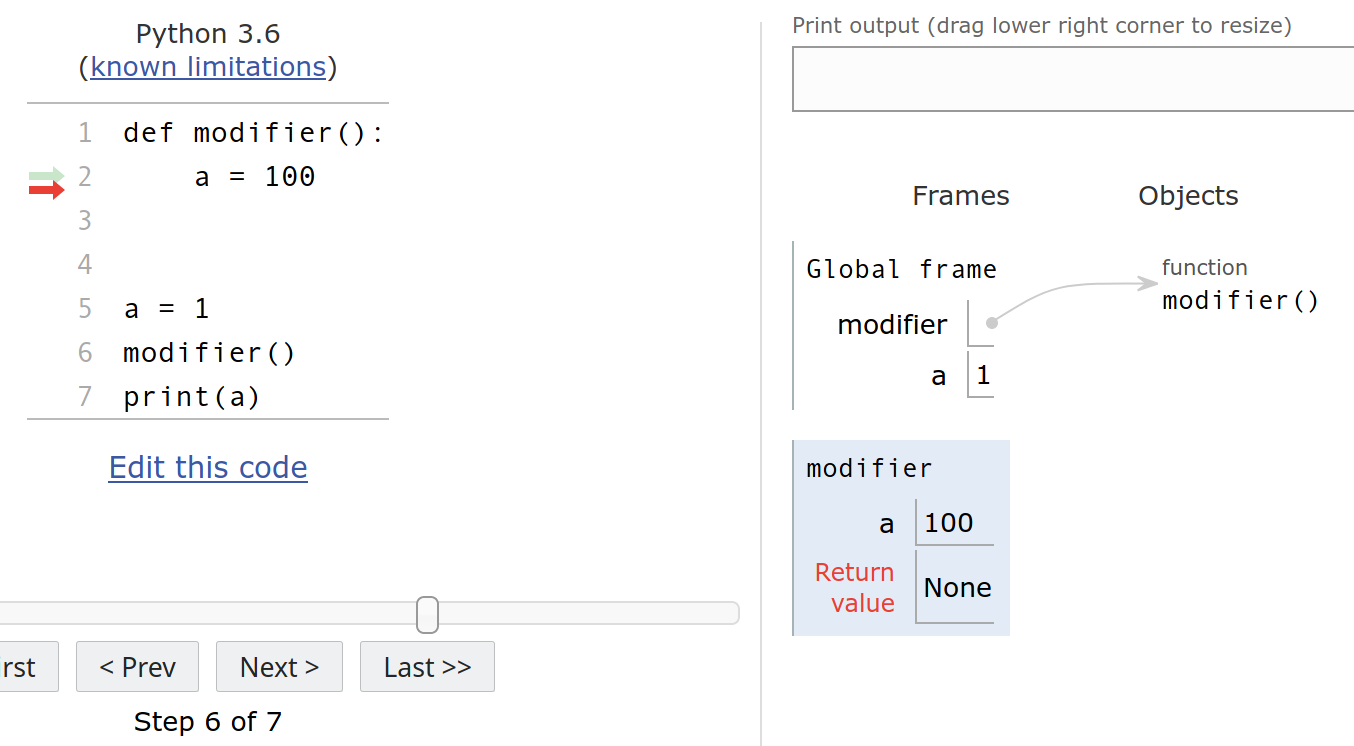
\includegraphics[width=0.75\linewidth]{img-var.png}
\end{center}

        \end{remarque}\begin{eleve}
    Qu'affiche l'exécution du code suivant ?

\begin{Shaded}
\begin{Highlighting}[]
\KeywordTok{def}\NormalTok{ incrementer(x):}
\NormalTok{    x }\OperatorTok{=}\NormalTok{ x }\OperatorTok{+} \DecValTok{1}
    \BuiltInTok{print}\NormalTok{(}\StringTok{"dans la fonction, x:"}\NormalTok{, x)}

\NormalTok{x }\OperatorTok{=} \DecValTok{1}
\BuiltInTok{print}\NormalTok{(}\StringTok{"au moment de l\textquotesingle{}appel, x:"}\NormalTok{, x)}
\NormalTok{incrementer(x)}
\BuiltInTok{print}\NormalTok{(}\StringTok{"après l\textquotesingle{}appel, x:"}\NormalTok{, x)}
\end{Highlighting}
\end{Shaded}
        
        \end{eleve}\begin{reponse}
    \begin{enumerate}
\def\labelenumi{\arabic{enumi}.}
\tightlist
\item
  Au moment de l'appel à la fonction \texttt{incrementer}, la variable
  \texttt{x} vaut 1. Un premier affichage indique donc
  \texttt{au\ moment\ de\ l\textquotesingle{}appel,\ x:\ 1}.
\item
  La appel à la fonction \texttt{incrementer} avec pour argument
  \texttt{x} a pour effet immédiat de créer une variable \textbf{locale}
  \texttt{x} qui est initialisée avec la valeur \texttt{1} contenue dans
  la variable \textbf{globale} \texttt{x}. Puis la première instruction
  de la fonction modifie cette variable \emph{locale} qui vaut
  maintenant \texttt{2}. Enfin, la deuxième instruction affiche la
  valeur de de cette variable \emph{locale} et affiche donc
  \texttt{dans\ la\ fonction,\ x:\ 2}.
\item
  La fonction se termine et la variable \emph{locale} \texttt{x}
  disparaît. En revanche, la variable globale \texttt{x} est toujours
  présente et n'a absolument pas été modifiée. Et la dernière
  instruction affiche \texttt{après\ l\textquotesingle{}appel,\ x:\ 1}.
\end{enumerate}

        \end{reponse}
    \hypertarget{sortie-anticipuxe9e}{%
\subsubsection{Sortie anticipée}\label{sortie-anticipuxe9e}}

    Dès que le mot clé \texttt{return} est rencontré, l'exécution de la
fonction s'arrête \textbf{immédiatement}.

La fonction renvoie alors le ou les résultats situés à droite du
mot-clé.
\begin{eleve}
    Qu'affiche le programme ci-dessous ?

\begin{Shaded}
\begin{Highlighting}[]
\KeywordTok{def}\NormalTok{ sortie(n):}
    \ControlFlowTok{if}\NormalTok{ n }\OperatorTok{\textgreater{}} \DecValTok{100}\NormalTok{:}
        \ControlFlowTok{return} \VariableTok{True}
    \ControlFlowTok{return} \VariableTok{False}

\BuiltInTok{print}\NormalTok{( (sortie(}\DecValTok{101}\NormalTok{), sortie(}\DecValTok{99}\NormalTok{)) )}
\end{Highlighting}
\end{Shaded}
        
        \end{eleve}\begin{reponse}
    Le programme affiche un n-uplet composé de (1) le résultat de l'appel à
\texttt{sortie(101)} et de (2) le résultat de l'appel à
\texttt{sortie(99)}.

Commençons par le (2). La fonction s'initialise avec \texttt{n} qui vaut
99. Comme 99 est inférieur à 100, on a la condition
\texttt{n\ \textgreater{}\ 100} qui est fausse. Le bloc conditionnel
n'est pas exécuté. Le programme \emph{saute} à la ligne 3 qui renvoie
\texttt{False}.

Pour le (1), la variable \texttt{n} est initialisée à 101. La condition
\texttt{n\ \textgreater{}\ 100} est vraie. Le bloc conditionnel est
exécuté. La ligne 2 est un renvoie qui \textbf{interrompt immédiatement}
le programme. La fonction renvoie la valeur \texttt{True}.

Pour conclure, le programme affiche le tuple : \texttt{(True,\ False)}.

        \end{reponse}
    \hypertarget{exercices}{%
\subsubsection{Exercices}\label{exercices}}
\begin{eleve}
    \textbf{Définir} une fonction \texttt{test\_Pythagore} qui prend trois
entiers \(a\), \(b\) et \(c\) en arguments et renvoie un booléen
indiquant si \(a^2 + b^2 = c^2\), ou \(b^2 + c^2 = a^2\) ou
\(c^2 + a^2 = b^2\).
        
        \end{eleve}\begin{eleve}
    \textbf{Définir} une fonction \texttt{valeur\_absolue} qui prend un
entier en argument et renvoie sa valeur absolue.
        
        \end{eleve}\begin{eleve}
    \textbf{Créer} une fonction \texttt{multiples} pour qu'elle prenne la
limite en argument plutôt que d'utiliser la valeur \(999\). En déduire
une fonction \texttt{multiples\_3\_ou\_5(borne\_sup)} qui renvoie la
somme des multiples de 3 ou 5 inférieurs ou égaux à \texttt{borne\_sup}.
        
        \end{eleve}\begin{eleve}
    \textbf{Écrire} une fonction \texttt{max2(a,\ b)} qui renvoie le plus
grand des deux entiers \texttt{a} et \texttt{b}.
        
        \end{eleve}\begin{eleve}
    En supposant la fonction \texttt{max2} précédente disponible,
\textbf{écrire} une fonction \texttt{max3(a,\ b,\ c)} qui utilise la
fonction \texttt{max2} de l'exercice précédent et qui renvoie le plus
grand des trois entiers \texttt{a}, \texttt{b}, \texttt{c}.
        
        \end{eleve}\begin{eleve}
    \textbf{Écrire} une fonction \texttt{puissance(x,\ k)} qui renvoie
\texttt{x} à la puissance \texttt{k} (utilisation de l'opérateur
\texttt{**} interdit ! évidemment\ldots). On utilisera une boucle
\texttt{for} pour faire le calcul.

On suppose que \(k\geq 0\) et on rappelle que \(x^0 = 1\).
        
        \end{eleve}\begin{eleve}
    \textbf{Écrire} une fonction \texttt{est\_bissextile(annee)} qui renvoie
un booléen indiquant si l'année \texttt{annee} est une année bissextile.

On rappelle qu'une année bissextile est une année multiple de 4 mais pas
de 100, ou multiple de 400.
        
        \end{eleve}\begin{eleve}
    \textbf{Écrire} une fonctions \texttt{nb\_jours\_annee(annee)} qui
renvoie le nombre de jour de l'année \texttt{annee}. La fonction
\texttt{est\_bissextile} de l'exercice précédent est disponible et vous
pouvez l'utiliser (ce qui est bien pratique quand même).
        
        \end{eleve}\begin{eleve}
    En supposant que le mois \texttt{mois} est un entier compris entre 1
(pour janvier) et 12 (décembre), \textbf{écrire} une fonction
\texttt{nb\_jours\_mois(annee,\ mois)} qui renvoie le nombre de jours
dans le mois \texttt{mois} de l'année \texttt{annee}. La fonction
\texttt{est\_bissextile} de l'exercice précédent est disponible (ce qui
est bien pratique).
        
        \end{eleve}\begin{eleve}
    En supposant les fonctions \texttt{nb\_jours\_annnee} et
\texttt{nb\_jours\_mois} disponibles, \textbf{écrire} une fonction
\texttt{nb\_jours(j\_debut,\ m\_debut,\ a\_debut,\ j\_fin,\ m\_fin,\ a\_fin)}
qui renvoie le nombre de jours compris entre deux dates données
(incluses).
        
        \end{eleve}

    % Add a bibliography block to the postdoc
    
    
    
\end{document}
